\newpage
\hypertarget{t2m close}{}
\subsection{Additional author handling}
\genHeader

\begin{itemize}

\item[$\blacktriangleright$] If your project's build succeeded, run the transformation\footnote{If you haven't already, read Part IV, Section 6 for details on to run a transformation} again and examine the successful forward output, 
\texttt{fwd.trg.xmi}, a little closer (Fig.~\ref{eclipse:generatedFwdTrsfm}).

\vspace{0.5cm}

\begin{figure}[htbp]
\begin{center}
  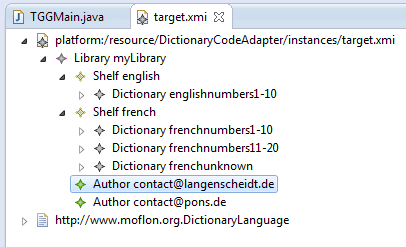
\includegraphics[width=0.7\textwidth]{eclipse_generatedForwardTransformation}
  \caption{\texttt{Dictionary} result of the forward transformation}
  \label{eclipse:generatedFwdTrsfm}
\end{center}
\end{figure} 

\vspace{0.5cm}

\item[$\blacktriangleright$] Your output may or may not resemble ours. In fact, there's a 50/50 chance that either a single or two \texttt{contact@pons.de} authors are created!
At run-time, the transformation has a choice between two rules to apply to a matched \texttt{authorNode}. 
The resulting choice is entirely random, meaning that your output is likely to be different each time you run the transformation. 
For a deterministic transformation, you would need to force a preferred decision. 

\noindent There are two ways to do this: 
\begin{enumerate}
\item At run-time, allowing users to decide for themselves what they would prefer to use, or 
\item At design-time, making the decision a part of the TGG specification.
\end{enumerate}

\vfill

\end{itemize}

\subsubsection{Option 1: Run-time decision}

The advantage with this option is that you give users the choice of what they prefer. 
Some users don't mind having multiple authors, while others might prefer a minimalist design. 
They can easily change their preference possibly on a case-by-case basis, by implementing a TGG rule \emph{configurator}.

\begin{itemize}

\item[$\blacktriangleright$] Implement and set the configurator to be used for the transformation as depicted in Fig.~\ref{eclipse:editTGGMain}.
Note how the possible alternatives are filtered using an \texttt{isRule} predicate to compare the name of each alternative with the preferred rule \texttt{NewAuthorRule} in this case.
As this degree of freedom concerning the creation or possible reuse of authors only arises in the forward direction, we do not need a similar configurator for the backward transformation.

\begin{figure}[htbp]
\begin{center}
  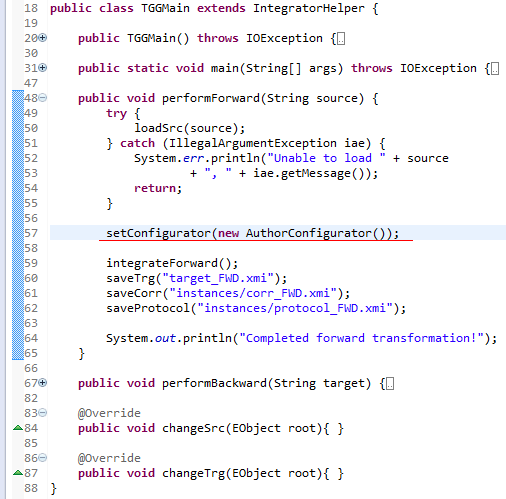
\includegraphics[width=0.9\textwidth]{eclipse_authorConfiguratorTGGMain}
  \caption{Setting the configurator to control the run-time decision}
  \label{eclipse:editTGGMain}
\end{center}
\end{figure}

\item[$\blacktriangleright$] Save and run the transformation a few times, using the integrator to confirm your preference is enforced each time.
You should now \emph{always} get two \texttt{contact@pons.de} authors using this configurator.
Try to change your preference and see the effect!

\end{itemize}

\subsubsection{Option 2: Design-time decision}

It is also possible to set a preference as part of the actual design of the transformation -- users will not be able to modify this. In our example, this
preference can be enforced using a NAC which checks to see if there is already an author with the same email in the library.

\begin{itemize}

\item[$\blacktriangleright$] Open and update either \texttt{NewAuthorRule} (visual) as shown in Fig.~\ref{ea:existingAuthorNAC} or edit the target domain in 
Eclipse (textual) as depicted in Fig.~\ref{eclipse:existingAuthorNAC}.

\begin{figure}[htbp]
\begin{center}
  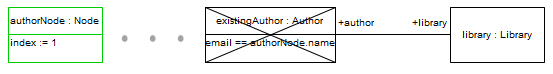
\includegraphics[width=\textwidth]{ea_NewAuthorRuleNAC}
  \caption{Adjust \texttt{NewAuthorRule} by adding a NAC}
  \label{ea:existingAuthorNAC}
\end{center}
\end{figure}

\vspace{0.5cm}

\begin{figure}[htbp]
\begin{center}
  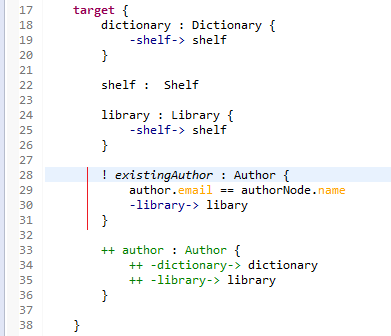
\includegraphics[width=0.7\textwidth]{eclipse_ForAllNewAuthorNAC}
  \caption{Add a NAC to \texttt{NewAuthorRule}}
  \label{eclipse:existingAuthorNAC}
\end{center}
\end{figure}

\vspace{0.5cm}

\item[$\blacktriangleright$] Save and rebuild the TGG, then run the transformation a few times. Confirm your preference is enforced each time -- With this NAC,
the configurator won't be given the chance to decide anymore!

\end{itemize}
